\section{Versuchsbedingungen}
Um in diesem Versuchsteil eine Anregung der naechsthoeheren Stufe zu erreichen, muss die Frank Hertz Roehre Umfunktioniert werden.
Dies wird durch das Zusammenschalten der beiden Gitter auf das gleiche Potential, und das absenken des Dampfdruckes erreicht.
Zum einen werden die Elektronen nun auf einer deutlich kuertzeren Strecke beschleunigt, was einerseits die Kollisionswahrscheinlichkeit waehrend der beschleunigung reduziert, andererseits ist der Dampfdruck niedriger, was nochmals die Stosswahrschinlichkeit verringert.
Im Raum zwischen Gitter 1 und 2 koennen die Elektronen nun stossen.
Um eine Gasentladung zu vermeiden, wird die Anzahl der Elektronen durch absenken der Heizspannung verringert.\\
\section{Beobachtungen}
Mit einer nach~\ref{Versuchsbedingungen} eingestellten Roehre laesst sich der in~\ref{fig:FrankHertz2} abgebildete Verlauf messen.
\begin{figure}
	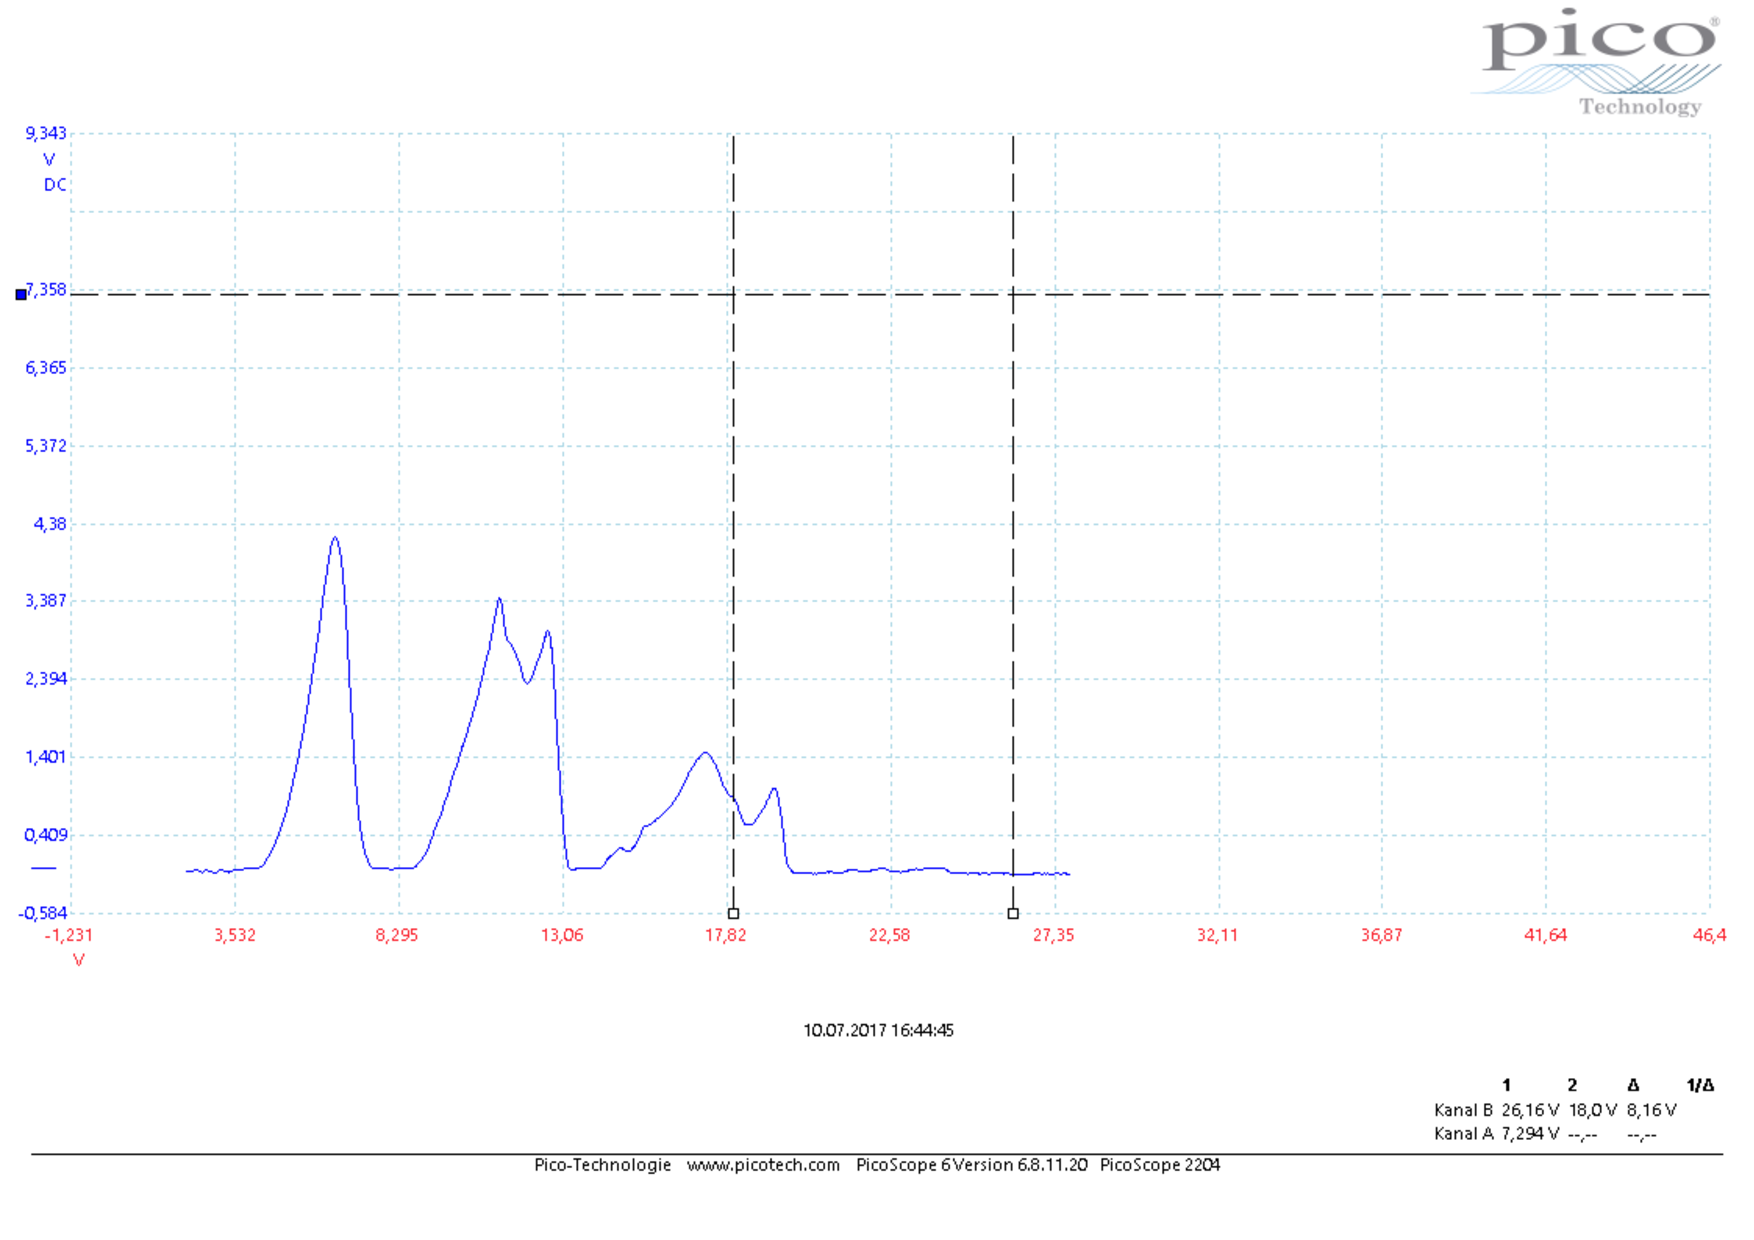
\includegraphics[width=\textwidth]{../Daten/Frank_Hertz_2.pdf}
	\caption{Frank Hertz kurve mit 1. und 2. Anregung}
	\label{fig:FrankHertz2}
\end{figure}
Man sieht in dem plot gut die Anregungen, welche Linearkombinationen der in \ref{tab:hgAnr} aufgelisteten Anregungen sind.
\begin{table}
	\centering
	\caption{Anregungsniveaus von Quecksilber}
	\begin{tabular}{l | c c}
		\toprule
		1. Anregung (a) & $6s^1S_0$ nach $6p^3P_1$ & 4,9V\\
		2. Anregung (b)& $6s^1S_0$ nach $6p^1P_1$ & 6,7V\\
	\end{tabular}
	\label{tab:hgAnr}
\end{table}
In~\ref{tab:hgAnrgem} sind die Verschiedenen Peaks mit den durch Vergleich ermittelten Anregungen aufgetragen.
An~\ref{tab:hgAnrgem} laesst sich auch gut erkennen, dass die Kurve um ca 2 V nach oben verschben ist.
Dies kann auf eine fehlerhafte Kalibrierung des Betriebsgeraetes zuueckgefuehrt werden.
\begin{table}
	\centering
	\caption{gemessene Anregungen von Quecksilber}
	\begin{tabular}{l | c c}
		Peak / Knick & $U_g$ in V& Anregung\\
		\midrule
		1 & 5,5 & a \\
		2 & 10,9 & 2 a \\
		3 & 12,3 & a + b \\
		4 & 14,5 & 2 b \\
		5 & 16,3 & 2 a + b \\
		6 & 19,0 & a + 2 b \\
	\end{tabular}
	\label{tab:hgAnrgem}
\end{table}
\section{Bemerkungen zur Einstellung des Versuches}
Die Einstellung des versuches ist in kleinen schritten durchgefuehrt worden da der Graph bereits fuer Aenderungen um ca 100 mV bereits grosse abweichungen zeigt.
Es wurden ca 15 Versuche gebraucht die fuer das Bild optimalen Einstellungen zu finden.
